\chapter{System Model} 		\label{sec_sys_model}
One of main contribution of this paper is the analytical evaluation of the saturation analysis of 802.11ax OFDMA-based random access, in the assumption of ideal channel conditions (i.e., no hidden terminals and capture). 
The Markov chain model of random access was first proposed by Bianchi for analyzing distributed coordination function\cite{bianchi2000performance}. 
Here, for the brand new ODFMA-based random access, we generate a new Markov chain model. 
In this analysis, we also generate three metrics, $n_s$ number of stations who succeed in contending in a stage, \textit{eff} self-defined system efficiency, and $D$ access delay of request frame. 

The analysis is divided into two parts. First is the Markov chain model to estimate the packet transmission probability $\tau$ and conditional collision probability $p$. 
Secondly, we express the three metrics as function of $\tau$. 
Table \ref{table_notation} is a list of all parameters and notations.

\begin{table}[!h]
\caption{Parameters and Notations}
\centering
\label{table_notation}
\begin{tabular}{c|l}
\hline
$n$						& $\#$ of stations \\
$OCW_{min}$ or $W_0$		& minimum OFDMA contention window \\
$M$						& $\#$ of RUs for random access \\
$m$						& maximum backoff level \\
$p$						& packet collision probability \\
$\tau$					& station's transmission probability \\
$n_s$					& $\#$ of successful stations in a stage \\
$N_{s\_station}$			& $\#$ of stages for a station to succeed in contending \\
$N_{s\_stage}$			& $\#$ of stages until a successful stage \\
\hline
\end{tabular}
\end{table}

\section{Packet Transmission Probability}
Since 802.11ax implements OFDMA-MU and corresponding trigger-based UL, AP won't contend with 802.11ax stations under this situation.
To estimate the performance of the OFDMA-based random access mechanism, we assume a saturated condition that each station always has packets to transmit as long as it accesses the channel.
In the first use case, each station will contend to send \textit{Buffer Status Report} (BSR), for convenience and easy understanding we call it request in the following context, for the data transmission later. 

With above illustration of OFDMA-based random access mechanism, a 20 MHz channel, which is a single user (SU) channel in legacy 802.11, can be divided into 9 subchannels, called resource unit (RU). Consider a fixed number $n$ of contending stations. 
$M$ represents the number of RU for random access in a stage. 
$W_i$ is the OFDMA contention window (OCW) at $i^{th}$ backoff level, with relationship $W_i = 2W_{i-1}+1$. Stations with OCW $W_i$ will randomly generate a backoff counter among range $[0,W_i]$.  

The bidimensional process $\lbrace s(t),b(t) \rbrace$, where $s(t)$ denotes the backoff level $(0,1\cdots ,m)$ of a given station at time $t$ and $b(t)$ denotes backoff time counter (i.e., OBO) for the station, will be modeled with Markov chain as in figure\ref{Markov}. 
Since states $\lbrace i,0\sim M \rbrace$ all means station could access RU, we could merge these states into one state, denoted by $\lbrace i, T \rbrace$. 

The model is based on the assumption that at each request transmission, and regardless of the number of retransmission suffered, each request frame collides with constant and independent probability $p$.

\begin{figure*}[!t]
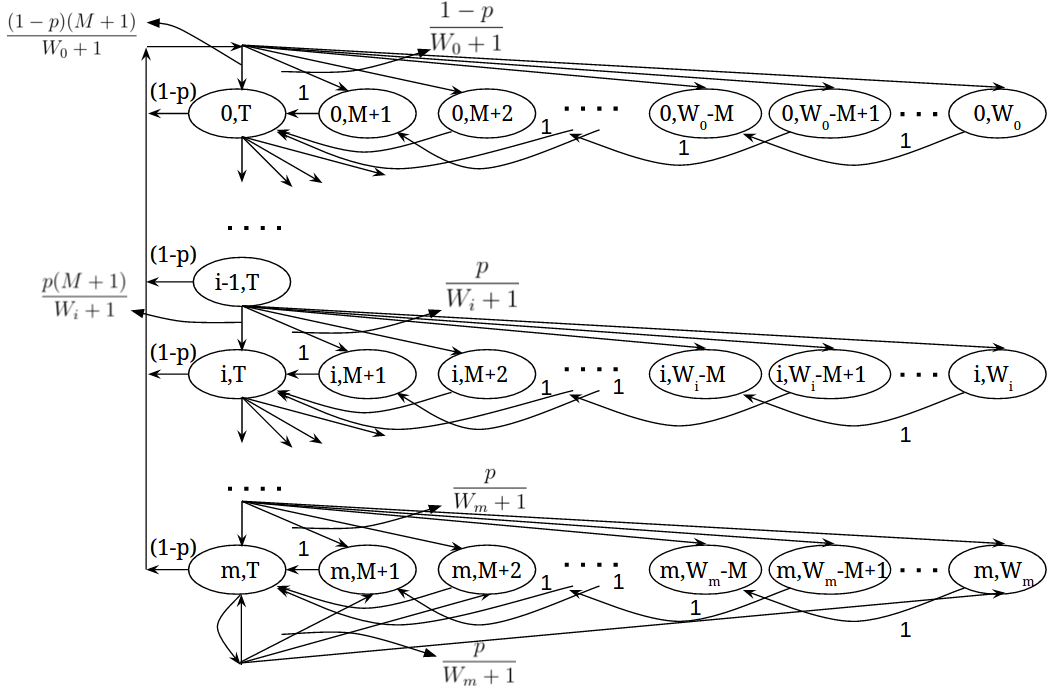
\includegraphics[scale=.45]{./figure/Markov_chain.png}
\caption{Markov Chain model for the backoff window size}
\label{Markov}
\end{figure*}

Let's assume $P\lbrace i_1, k_1|i_0,k_0\rbrace = P\lbrace s(t+1) = i_1, b(t+1)= k_1|s(t) = i_0, b(t) = k_0\rbrace $. In this Markov Chain, the only non null one-step transition probabilities are 
\begin{align}
\left\lbrace
\begin{array}{lll}
P\lbrace i, T | i, k \rbrace = 1  						& k\in [M+1,2M]			& i \in [0,m]\\ [3pt]
P\lbrace i, k-M | i, k \rbrace = 1  						& k\in [2M+1,W_i]   		& i \in [0,m]\\ [3pt]
P\lbrace 0, k | i, T \rbrace = \frac{1-p}{W_0+1}  		& k\in [M+1,W_0]			& i \in [0,m]\\ [3pt]
P\lbrace 0, T | i, T \rbrace = \frac{(1-p)(M+1)}{W_0+1}  &						& i \in [0,m]\\ [3pt]
P\lbrace i, k | i-1, T \rbrace = \frac{p}{W_i+1} 		& k\in [M+1,W_i] 		& i \in [1,m]\\ [3pt]
P\lbrace i, T | i-1, T \rbrace = \frac{p(M+1)}{W_i+1}    &  						& i \in [1,m]\\ [3pt]
P\lbrace m, k | m, T \rbrace = \frac{p}{W_m+1} 		 	& k\in [M+1,W_m] 		& \\ [3pt]
P\lbrace m, k | m, T \rbrace = \frac{p(M+1)}{W_m+1}
\end{array}
\right.
\label{trans_prob}
\end{align}
The first and second equations in \ref{trans_prob} accounts for the fact that in a trigger frame stage for random access, the backoff counter maintained by stations will decrease the number of RUs for random access. 
The third and fourth equation represents that after a successful contention, stations will reset the contention window size to initial window size and uniformly generate a backoff value among $[0,W_0]$, since $T = [0,M]$, the transition probability to $\lbrace i, T \rbrace$ is $M+1$ times of that to $\lbrace i, k \rbrace$. 
For the fifth and sixth equations, they represents when a failure contention occurs, the contention window size will be doubled. 
The last two equation is situation of failure contention at the maximum backoff level.

Let $b_{i,k} = \lim_{t\rightarrow \infty} P\lbrace s(t) = i, b(t) = k\rbrace,\ i\in [0,m], \ k \in [0,W_i]$ be the stationary distribution of the Markov chain. Then we show the steady state for the Markov Chain.
First,  for $k = T$
\begin{align}
b_{i-1,T}\cdot p = b_{i,T} 		\rightarrow b_{i,T} = p^i b_{0,T}, \quad 0\leq i < m\\
b_{m-1,T}\cdot p = (1-p) b_{m,T}	\rightarrow b_{m,T} = \frac{p^m}{1-p}b_{0,T}.
\label{biT}
\end{align}

Then,
\begin{align}
&b_{i,k} =  \nonumber \\
&
\begin{cases}
(\lfloor \frac{W_0-k}{M} \rfloor+1)\frac{(1-p)}{W_0+1}\sum_{i=0}^m b_{i,T}, \  M+1\leq k\leq W_0,\ i = 0\\[3pt]
(\lfloor \frac{W_i-k}{M} \rfloor+1)\frac{p}{W_i+1}b_{i-1,T}, 				\	 M+1 \leq k\leq W_i, \ 0<i<m \\[3pt]
(\lfloor \frac{W_m-k}{M} \rfloor+1)\frac{p}{W_m+1} (b_{m-1,T}+b_{m,T}), 	
\end{cases}\nonumber
\\ &\qquad \qquad \qquad \qquad \quad \qquad \qquad M+1 \leq k\leq W_m, \quad i = m \nonumber \\
\label{steady_prob}
\end{align}

From equation \ref{biT}, we have $\sum_{i=0}^m b_{i,T}= \frac{b_{0,T}}{1-p}$; sum the equation \ref{steady_prob} respectively, we obtain equation \ref{part_sum}.  
\begin{figure*}[!b]
\begin{align}
\begin{cases}
\sum_{k=M+1}^{W_0} b_{0,k} = \frac{b_{0,T}}{W_0+1}\left(-\frac{M}{2}\left\lfloor \frac{W_0}{M}\right\rfloor ^2 + \left(W_0-\frac{M}{2}\right)\left\lfloor \frac{W_0}{M} \right\rfloor \right) \\[8pt]
\sum_{i=1}^{m-1}\sum_{k=M+1}^{W_i} b_{i,k} = \frac{b_{0,T}}{W_0+1}\left(\frac{p}{2}\right)^i \left(-\frac{M}{2}\left\lfloor \frac{W_i}{M}\right\rfloor ^2 + \left(W_i-\frac{M}{2}\right)\left\lfloor \frac{W_i}{M} \right\rfloor \right) \\[8pt]
\sum_{k=M+1}^{W_m} b_{m,k} = \frac{b_{0,T}}{W_0+1}\frac{(\frac{p}{2})^m}{1-p}\left(-\frac{M}{2}\left\lfloor \frac{W_m}{M}\right\rfloor ^2 + \left(W_m-\frac{M}{2}\right)\left\lfloor \frac{W_m}{M} \right\rfloor \right) 
\end{cases}
\label{part_sum}
\end{align}
\end{figure*}

Let $X_i = -\frac{M}{2}\left\lfloor \frac{W_i}{M}\right\rfloor ^2 + \left(W_i-\frac{M}{2}\right)\left\lfloor \frac{W_i}{M} \right\rfloor$. Then we sum all the states to have equation \ref{total_sum2}.
\begin{figure*}[!b]
\begin{align}
1 &= \sum_{i=0}^m \sum_{k=0}^{W_i}b_{i,k} 
 = \frac{b_{0,T}}{W_0+1}\left( X_0 + \sum_{i=1}^{m-1}X_i\left( \frac{p}{2}\right)^i + X_m\frac{\left( \frac{p}{2}\right)^m}{1-p}\right) + \frac{b_{0,T}}{1-p}\label{total_sum}\\
& = b_{0,T}\left( \frac{(1-p)X_0+(1-p) \sum_{i=1}^{m-1}X_i\left( \frac{p}{2}\right)^i+X_m\left( \frac{p}{2}\right)^m+W_0+1}{(W_0+1)(1-p)}\right)\label{total_sum2}
\end{align}
\end{figure*}

We can now express $\tau$, the probability of a station transmit a request at a randomly selected stage.

\begin{align}
\label{tau_general}
&\tau = \sum_{i=0}^m b_{i,T} = \frac{b_{0,T}}{1-p} = \nonumber \\
&\frac{W_0+1}{W_0+1+(1-p)X_0+(1-p) \sum_{i=1}^{m-1}X_i\left( \frac{p}{2}\right)^i+X_m\left( \frac{p}{2}\right)^m}
\end{align}

For $m=0$, check equation \ref{total_sum}, the terms containing $X_i, i>0$ will disappear, and $b_{0,T}/(1-p)$ will just be $b_{0,T}$.
Thus, equation \ref{total_sum2} will be simplified to 
\begin{align}
1 = b_{0,T}\left( \frac{W_0+1+X_0}{W_0+1}\right),
\end{align}
thereby, 
\begin{align}
\tau = b_{0,T} = \frac{W_0+1}{W_0+1+X_0}.
\label{tau_W0}
\end{align}
Thus $\tau$ is independent with $n$, number of contending stations.

On the other hand, conditional collision probability $p$ is the probability that no other stations select the same RU to transmit request. So we have 
\begin{align}
\label{p_ax}
p = 1-\left( 1-\frac{\tau}{M} \right)^{n-1}.
\end{align}
Rewrite the equation \ref{p_ax}, $\tau^\star = \left(1-(1-p)^\frac{1}{n-1} \right)M$. 
To obtain transmission probability $\tau$ and conditional probability $p$, we need to find solutions to group of equations \ref{tau_general} and \ref{p_ax}.
$\tau^\star(p)$ is a monotonically increasing function. 
Though $\tau(p)$ is hard to determine the monotonicity from the expression of equation \ref{tau_general} with respect to $p$. 
We justify the monotonic decrease of function \ref{tau_general} with numerical method. 
Also, $\tau(0) = \frac{W_0+1}{W_0+1+X_0}> \tau^\star(0) = 0$.
And $\tau(1) < \tau^\star(1) = M$. We find the only solution with numerical method.



\section{Random Access Efficiency}
With the transmit probability, we could easily estimate efficiency of random access mechanism. 
Firstly, find expected number of stations who succeed in contending to transmit request at a stage, which is denoted with $E[n_s]$. 
Extending $n_s$, we define a system efficiency as an important metric.
Secondly, we are interested in the access delay of request frame. 
In another word, say how many stages needed for a station to succeed in contending, denoted by $N_{s\_station}$.
What's more, another interesting metric is how many stages are elapsed until a successful stage, which means at least one station succeed in contending in the stage. This metric is a concept similar to "delay" in the second use case of OFDMA-based random access. We represent it with $N_{s\_stage}$. It helps design whole MU UL transmission procedure. 
Here, our concern is mainly on first two metrics which are purely related to random access procedure. The third metric is only expressed in the subsection of access delay, not being discussed later. 

\subsection{$n_s$ and System Efficiency}
What we care in the random access is that how many stations contend successfully in a single stage, denoted by $n_s$.
Given transmission probability $\tau$ and conditional collision probability $p$, we could obtain probability that a station succeeds in contending in a stage, $P_{s\_station} = \tau (1-p)$.
Then, with equation \ref{p_ax}, $E[n_s]$ is easily computed as follows. 
\begin{align}
\label{equ_ns}
E[n_s] &= n P_{s\_station} \nonumber \\
		&= n\tau (1-p) \nonumber \\
		&= n\tau (1-\frac{\tau}{M})^{n-1}
\end{align}

Furthermore, normalizing $n_s$, system efficiency here is defined as 
\begin{align}
\label{eff_def}
\textit{eff}\ (\tau) &= \frac{E[\text{number of successful stations in a given stage}]}{\text{number of RUs for random access in a stgae}} \nonumber\\
					 &=\frac{E[n_s]}{M} \nonumber \\
					 &= \frac{n\tau(1-\frac{\tau}{M})^{n-1}}{M}.
\end{align}

Both two metrics are our concerns. Another metric, access delay, is derived in next subsection.
With all these metrics, we could evaluate the performance later.

	
\subsection{Access Delay}
$N_{s\_station}$, the random variable of how many stages are needed for a station to succeed in contending in a stage follows geometric distribution with parameter $P_{s\_station}$, which is obtained just now.  
Then the expected value of access delay of request frame, $E[D]$, is 
\begin{align}
\label{equ_delay}
E[D] = E[N_{s\_station}] = \frac{1}{\tau (1-\frac{\tau}{M})^{n-1}}.
\end{align}

Then another interesting metric which is not our focus, denoted by $N_{s\_stage}$, that how many stages are elapsed until a successful stage. 
We could firstly obtain $P_{s\_stage}$, the probability of a successful stage, which means at least one station succeed in contending in the stage.

\begin{align}
P_{s\_stage} &= 1-P\lbrace n_s = 0\rbrace \nonumber \\
	&= 1-(1-P_{s\_station})^n \nonumber\\
	&= 1-(1-\tau(1-p))^n
\end{align} 	 
Since $N_{s\_stage}$ follows geometric distribution with parameter $P_{s\_stage}$,  
\begin{align}
E[N_{s\_stage}] &= \frac{1}{P_{s\_stage}}  \nonumber \\
			&= \frac{1}{1-(1-\tau(1-p))^n}
\end{align} 

In a word, we focus on three metrics: number of successful stations in a stage by $n_s$, system efficiency by $E[n_s]/M$ and access delay given by $N_{s\_station}$. 
Actually, only two variables are concerned, $n_s$ and $N_{s\_station}$. However, $n_s$ and its normalized value are both meaningful, which we will explain in following sections.


\section{Model Validation} 		\label{sec_model_val}
To validate the Markov chain model, we run a simulation using C language according to the settings of 802.11ax random access illustration. 
We run the simulation with variety of parameter sets $\lbrace M, m, OCW_{min}\rbrace$ and collects the information of the two variables, $n_s$ and $N_{s\_station}$. 
The validation is given in both figure \ref{validation} and table \ref{table_val}. 
The results show that the Markov model precisely predict the behavior of the OFDMA-based random access.
\begin{table}[!h]
\caption{Analysis versus simulation: $n_s$ and access delay with $m=3,M=9,OCW_{min} = 15$}
\label{table_val}
\begin{center}
\begin{tabular}{c|c|c}
\hline
$n_s$ 	& analysis 	& simulation \\
\hline
$n=1$ 	& 0.72727  	& 0.72728 \\
$n=5$ 	& 2.23001	& 2.22335 \\
$n=10$	& 2.88954	& 2.88546 \\
$n=20$	& 3.29798	& 3.29857 \\
\hline
delay	& analysis	& simulation \\
\hline
$n=1$ 	& 1.37500  	& 1.37499 \\
$n=5$ 	& 2.24214	& 2.24886 \\
$n=10$	& 3.46075	& 3.46565 \\
$n=20$	& 6.06432	& 6.06323 \\
\hline
\end{tabular}
\end{center}
\end{table}

\begin{figure}[!h]
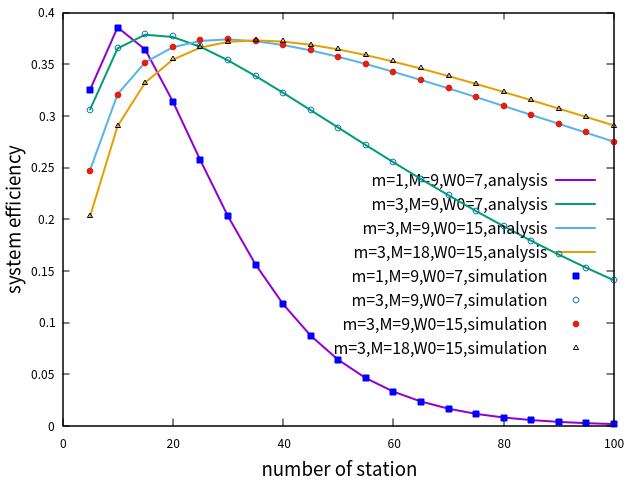
\includegraphics[scale=0.54]{./figure/multiple_parameter.png}
\caption{System efficiency: Analysis versus Simulation}
\label{validation}
\end{figure}